\documentclass{beamer}

\usepackage{focs-slides}
\usepackage{listings}

\title{Music Intelligence at Million-Song Scale}
\author{p1team02 $-$ Jiang Ruiyu, Li Zhiyuan, Yao Yunxiang, Zhang Jingkai}
\date{Summer 2026}
\course{ECE472}

\addbibresource{slides.bib}
\addbibresource{model_refs.bib}
\addbibresource{model_refs_story.bib}


% Section 1, 2, 4 -----------------------------
\definecolor{projectteal}{HTML}{236B65}
\definecolor{summaryred}{HTML}{B64E3C}
\definecolor{summaryfill}{HTML}{F5DDD8}
\definecolor{audioblue}{HTML}{4E79A7}
\definecolor{audiofill}{HTML}{DDEAF5}
\definecolor{distancegold}{HTML}{D1495B}
\definecolor{distancegoldfill}{HTML}{F7E4E7}
\definecolor{frontierpurple}{HTML}{7A5195}
\definecolor{frontierfill}{HTML}{EADFF2}


% Section 3 -----------------------------------
\definecolor{projectblue}{HTML}{3E7198}
\definecolor{projectpurple}{HTML}{76689A}
\definecolor{projectgold}{HTML}{D1495B}
\definecolor{projectink}{HTML}{173A38}


\colortheme{projectteal}

\lstdefinestyle{projectsql}{
	language=SQL,
	basicstyle=\ttfamily\scriptsize,
	keywordstyle=\color{structbgcolor}\bfseries,
	commentstyle=\color{black!55}\itshape,
	stringstyle=\color{structbgcolor!70!black},
	backgroundcolor=\color{structbgcolor!8},
	rulecolor=\color{structbgcolor!65},
	frame=single,
	framerule=.5pt,
	framesep=4pt,
	xleftmargin=0pt,
	xrightmargin=0pt,
	aboveskip=0pt,
	belowskip=0pt,
	columns=fullflexible,
	keepspaces=true,
	breaklines=true,
	breakatwhitespace=true,
	showstringspaces=false,
	tabsize=2
}

\lstnewenvironment{sqlcode}[1][]
	{\lstset{style=projectsql,#1}}
	{}

\begin{document}

\maketitle

\toc{enum}

\section{Drill Queries}

\begin{frame}[t]{From HDF5 to Parquet}

\centering
\begin{tikzpicture}[
	font=\small,
	flow/.style={->,>=stealth,line width=1.1pt},
	source/.style={rounded corners=2pt,minimum width=2.8cm,minimum height=1.35cm,
		align=center,line width=1.2pt,inner sep=7pt},
	table/.style={rounded corners=2pt,align=left,line width=1.2pt,inner sep=7pt},
	heading/.style={font=\normalsize\bfseries,text=black!55}
]
	\node[heading] at (0,2.75) {MSD};
	\node[heading] at (4.1,2.75) {PARQUET};
	\node[heading] at (8.4,2.75) {DRILL};

	\node[source,fill=summaryfill,draw=summaryred,text=summaryred] (summary) at (0,0) {
		\textbf{Summary HDF5}\\[2pt]
		\scriptsize\texttt{AdditionalFiles/}\\[-1pt]
		\scriptsize\texttt{msd\_summary\_file.h5}
	};

	\node[source,fill=audiofill,draw=audioblue,text=audioblue] (raw) at (0,-3.60) {
		\textbf{Per-track HDF5}\\[2pt]
		\scriptsize\texttt{data/.../*.h5}
	};

	\node[table,draw=summaryred,text width=3.0cm] (songs) at (4.1,0) {
		\centering\textbf{songs}\par
		\vspace{2pt}
		{\scriptsize
		\renewcommand{\arraystretch}{.95}
		\begin{tabular}{@{}l@{}}
			\\ \texttt{track\_id} \\
			\texttt{year} \\
			\texttt{title} \\
			\texttt{artist\_id} \\
			\texttt{artist\_name} \\
			\texttt{song\_hotttnesss} \\
			\texttt{duration} \\
			\texttt{tempo} \\
			\texttt{release\_7digitalid} \\
			\texttt{release}
		\end{tabular}}
	};

	\node[table,draw=audioblue,text width=3.0cm] (audio) at (4.1,-3.60) {
		\centering\textbf{audio}\par
		\vspace{2pt}
		{\scriptsize
		\renewcommand{\arraystretch}{.95}
		\begin{tabular}{@{}l@{}}
			\\ \texttt{track\_id} \\
			\texttt{energy}
		\end{tabular}}
	};

	\node[rounded corners=2pt,fill=structbgcolor!18,draw=structbgcolor,
		minimum width=2.4cm,minimum height=1.45cm,align=center,
		text=structbgcolor!55!black,line width=1.2pt] (drill) at (8.4,-1.8) {
		\textbf{Apache Drill}\\[3pt]
		\scriptsize SQL queries
	};

	\draw[flow,draw=summaryred] (summary.east) -- (songs.west);
	\draw[flow,draw=audioblue] (raw.east) -- (audio.west);
	\draw[flow,draw=summaryred] (songs.east) -| (drill.north);
	\draw[flow,draw=audioblue] (audio.east) -| (drill.south);
\end{tikzpicture}

\end{frame}

\begin{frame}{Results}

\centering
\begin{tikzpicture}[
	result/.style={align=left,text width=5.05cm},
	label/.style={font=\scriptsize\bfseries,text=black!55}
]
	\draw[black!18,line width=.8pt] (0,-3.40) -- (0,2.55);
	\draw[black!18,line width=.8pt] (-5.45,-.12) -- (5.45,-.12);

	\node[result,anchor=north west] at (-5.45,2.25) {
		{\usebeamerfont*{normal text}\scriptsize\bfseries\color{black!55}
		VALID YEAR RANGE}\par
		\vspace{.42cm}
		{\LARGE\bfseries\color{structbgcolor}1922--2011}
	};

	\node[result,anchor=north west] at (.4,2.25) {
		{\usebeamerfont*{normal text}\scriptsize\bfseries\color{black!55}
		EXTREME SONG}\par
		\vspace{.36cm}
		{\Large\bfseries ``Jingle Bell Rock''}\par
		\vspace{.08cm}
		{\small Bobby Helms}
	};

	\node[result,anchor=north west] at (-5.45,-.72) {
		{\usebeamerfont*{normal text}\scriptsize\bfseries\color{black!55}
		ALBUM WITH MOST TRACKS}\par
		\vspace{.32cm}
		{\LARGE\bfseries\color{structbgcolor}85}
		{\large\bfseries\ tracks}\par
		\vspace{.1cm}
		{\small ``First Time In A Long Time:\par
		The Reprise Recordings''}
	};

	\node[result,anchor=north west] at (.4,-.72) {
		{\usebeamerfont*{normal text}\scriptsize\bfseries\color{black!55}
		LONGEST SONG}\par
		\vspace{.32cm}
		{\LARGE\bfseries\color{structbgcolor}3034.91}
		{\large\bfseries\ s}\par
		\vspace{.1cm}
		{\large\bfseries ``Grounation''}\par
		{\small Mystic Revelation of Rastafari}
	};
\end{tikzpicture}

\end{frame}


\section{Artist Distance}

\begin{frame}{Supports song recommendation}

\centering
\makebox[\textwidth][c]{%
\begin{tikzpicture}[
	xscale=1.12,
	yscale=.88,
	>=stealth,
	artistedge/.style={->,line width=1.1pt,draw=black!38},
	inactiveedge/.style={->,line width=.8pt,draw=black!13},
	frontieredge/.style={->,line width=1.5pt,draw=frontierpurple},
	songedge/.style={line width=.62pt,draw=black!24},
	inactivesongedge/.style={line width=.55pt,draw=black!11},
	frontiersongedge/.style={line width=1.15pt,draw=frontierpurple},
	artist/.style={circle,minimum size=.72cm,draw=projectteal,line width=1.15pt,
		fill=projectteal!48},
	inactiveartist/.style={artist,draw=black!18,fill=white},
	frontierartist/.style={artist,draw=frontierpurple,line width=1.9pt,
		fill=frontierfill},
	song/.style={circle,minimum size=.19cm,inner sep=0pt,line width=.65pt},
	inactivesong/.style={song,draw=black!18,fill=white},
	targetsong/.style={song,draw=summaryred!80!black,fill=summaryred},
	dzero/.style={song,draw=summaryred,fill=summaryred!35},
	done/.style={song,draw=distancegold,fill=distancegoldfill},
	dtwo/.style={song,draw=audioblue,fill=audioblue!48},
	frontiermark/.style={song,draw=frontierpurple,line width=1.2pt,
		fill=frontierfill},
	legend/.style={font=\scriptsize\bfseries,text=black!58,anchor=west},
	status/.style={font=\scriptsize\bfseries,text=black}
]
	\path[use as bounding box] (-4.55,-4.95) rectangle (4.55,3.55);

	\alt<1>{\def\rootartiststate{inactiveartist}}
		{\alt<2>{\def\rootartiststate{frontierartist}}
			{\def\rootartiststate{artist}}}
	\alt<1-2>{\def\doneartiststate{inactiveartist}}
		{\alt<3>{\def\doneartiststate{frontierartist}}
			{\def\doneartiststate{artist}}}
	\alt<1-3>{\def\dtwoartiststate{inactiveartist}}
		{\alt<4>{\def\dtwoartiststate{frontierartist}}
			{\def\dtwoartiststate{artist}}}
	\alt<1-2>{\def\rootedgestate{inactiveedge}}
		{\alt<3>{\def\rootedgestate{frontieredge}}
			{\def\rootedgestate{artistedge}}}
	\alt<1-3>{\def\doneedgestate{inactiveedge}}
		{\alt<4>{\def\doneedgestate{frontieredge}}
			{\def\doneedgestate{artistedge}}}
	\alt<1-4>{\def\dtwoedgestate{inactiveedge}}
		{\alt<5>{\def\dtwoedgestate{frontieredge}}
			{\def\dtwoedgestate{artistedge}}}
	\alt<1-2>{\def\dzerosongstate{inactivesong}}
		{\def\dzerosongstate{dzero}}
	\alt<1-3>{\def\donesongstate{inactivesong}}
		{\def\donesongstate{done}}
	\alt<1-4>{\def\dtwosongstate{inactivesong}}
		{\def\dtwosongstate{dtwo}}
	\alt<1>{\def\targetedgestate{inactivesongedge}}
		{\alt<2>{\def\targetedgestate{frontiersongedge}}
			{\def\targetedgestate{songedge}}}
	\alt<1-2>{\def\dzeroedgestate{inactivesongedge}}
		{\def\dzeroedgestate{songedge}}
	\alt<1-3>{\def\donesongedgestate{inactivesongedge}}
		{\def\donesongedgestate{songedge}}
	\alt<1-4>{\def\dtwosongedgestate{inactivesongedge}}
		{\def\dtwosongedgestate{songedge}}

	\node[\rootartiststate] (root) at (0,0) {};
	\node[\doneartiststate] (aone) at (-2.0,1.0) {};
	\node[\doneartiststate] (atwo) at (.8,1.65) {};
	\node[\doneartiststate] (athree) at (2.0,-.55) {};
	\node[\doneartiststate] (afour) at (-1.25,-1.65) {};
	\node[\dtwoartiststate] (aoneone) at (-3.65,1.95) {};
	\node[\dtwoartiststate] (aonetwo) at (-3.8,.35) {};
	\node[\dtwoartiststate] (atwoone) at (-.1,2.8) {};
	\node[\dtwoartiststate] (atwotwo) at (2.1,2.65) {};
	\node[\dtwoartiststate] (athreeone) at (3.55,.35) {};
	\node[\dtwoartiststate] (athreetwo) at (3.45,-1.7) {};
	\node[\dtwoartiststate] (afourone) at (-2.8,-2.75) {};
	\node[\dtwoartiststate] (afourtwo) at (.05,-2.95) {};

	\foreach \from/\to in {
		root/aone,root/atwo,root/athree,root/afour}
		\draw[\rootedgestate] (\from) -- (\to);
	\foreach \from/\to in {
		aone/aoneone,aone/aonetwo,
		atwo/atwoone,atwo/atwotwo,
		athree/athreeone,athree/athreetwo,
		afour/afourone,afour/afourtwo}
		\draw[\doneedgestate] (\from) -- (\to);
	\foreach \from/\to in {
		atwoone/aone,
		atwotwo/athreeone}
		\draw[\dtwoedgestate] (\from) -- (\to);
	\draw[\doneedgestate,<->] (aone) -- (atwo);
	\foreach \from/\to in {
		aonetwo/afourone,
		athreetwo/afourtwo}
		\draw[\dtwoedgestate,<->] (\from) -- (\to);

	\node[targetsong] (query) at (-.58,-.38) {};
	\node[\dzerosongstate] (rzeroone) at (.52,.42) {};
	\node[\dzerosongstate] (rzerotwo) at (.66,-.16) {};
	\node[\dzerosongstate] (rzerothree) at (.08,.65) {};
	\draw[\targetedgestate] (root) -- (query);
	\foreach \songname in {rzeroone,rzerotwo,rzerothree}
		\draw[\dzeroedgestate] (root) -- (\songname);

	\foreach \artist/\one/\xone/\yone/\two/\xtwo/\ytwo/\three/\xthree/\ythree in {
		aone/aonea/-2.18/1.62/aoneb/-2.67/.98/aonec/-1.72/.44,
		atwo/atwoa/1.42/1.32/atwob/1.18/.98/atwoc/1.58/1.75,
		athree/athreea/1.54/-1.08/athreeb/2.28/-1.16/athreec/2.57/-.72,
		afour/afoura/-.68/-1.82/afourb/-1.14/-2.25/afourc/-1.82/-1.92}
	{
		\node[\donesongstate] (\one) at (\xone,\yone) {};
		\node[\donesongstate] (\two) at (\xtwo,\ytwo) {};
		\node[\donesongstate] (\three) at (\xthree,\ythree) {};
		\foreach \songname in {\one,\two,\three}
			\draw[\donesongedgestate] (\artist) -- (\songname);
	}

	\foreach \artist/\one/\xone/\yone/\two/\xtwo/\ytwo/\three/\xthree/\ythree in {
		aoneone/aoneonea/-4.16/2.34/aoneoneb/-4.24/1.82/aoneonec/-3.70/2.52,
		aonetwo/aonetwoa/-4.34/.67/aonetwob/-4.36/.16/aonetwoc/-3.84/-.27,
		atwoone/atwoonea/-.58/3.22/atwooneb/.04/3.42/atwoonec/.43/3.17,
		atwotwo/atwotwoa/1.72/3.15/atwotwob/2.38/3.20/atwotwoc/2.70/2.73,
		athreeone/athreeonea/4.08/.72/athreeoneb/4.20/.22/athreeonec/3.80/-.22,
		athreetwo/athreetwoa/4.02/-1.35/athreetwob/4.08/-1.91/athreetwoc/3.43/-2.30,
		afourone/afouronea/-3.35/-3.14/afouroneb/-2.77/-3.40/afouronec/-2.24/-3.10,
		afourtwo/afourtwoa/-.38/-3.40/afourtwob/.28/-3.47/afourtwoc/.65/-3.10}
	{
		\node[\dtwosongstate] (\one) at (\xone,\yone) {};
		\node[\dtwosongstate] (\two) at (\xtwo,\ytwo) {};
		\node[\dtwosongstate] (\three) at (\xthree,\ythree) {};
		\foreach \songname in {\one,\two,\three}
			\draw[\dtwosongedgestate] (\artist) -- (\songname);
	}

	\only<2>{
		\node[status] at (0,-4.72) {Initialize: frontier $=$ source artist};
	}
	\only<3>{
		\node[status] at (0,-4.72) {After $d=0$: frontier $=$ distance 1};
	}
	\only<4>{
		\node[status] at (0,-4.72) {After $d=1$: frontier $=$ distance 2};
	}
	\only<5>{
		\node[status] at (0,-4.72) {No new artists: frontier empty};
	}
	\only<6>{\coordinate (finalstate) at (0,0);}

	\node[targetsong] at (-3.425,-4.12) {};
	\node[legend] at (-3.255,-4.12) {target};
	\only<2-4>{
		\node[frontiermark] at (-1.875,-4.12) {};
		\node[legend] at (-1.705,-4.12) {frontier};
	}
	\only<3-6>{
		\node[dzero] at (-.325,-4.12) {};
		\node[legend] at (-.155,-4.12) {$d=0$};
	}
	\only<4-6>{
		\node[done] at (1.225,-4.12) {};
		\node[legend] at (1.395,-4.12) {$d=1$};
	}
	\only<5-6>{
		\node[dtwo] at (2.775,-4.12) {};
		\node[legend] at (2.945,-4.12) {$d=2$};
	}
\end{tikzpicture}
}

\end{frame}

\begin{frame}{Parallel execution}

\centering
\begin{tikzpicture}[
	>=stealth,
	artist/.style={circle,minimum size=.58cm,inner sep=0pt,draw=projectteal,
		line width=1.05pt,fill=projectteal!48},
	frontierartist/.style={artist,draw=frontierpurple,line width=1.7pt,
		fill=frontierfill},
	partitionone/.style={artist,draw=audioblue,fill=audiofill},
	partitiontwo/.style={artist,draw=distancegold,fill=distancegoldfill},
	partitionthree/.style={artist,draw=summaryred,fill=summaryfill},
	partitiononefrontier/.style={partitionone,draw=frontierpurple,line width=1.7pt},
	partitiontwofrontier/.style={partitiontwo,draw=frontierpurple,line width=1.7pt},
	partitionthreefrontier/.style={partitionthree,draw=frontierpurple,line width=1.7pt},
	futureartist/.style={artist,draw=black!22,fill=white},
	edge/.style={->,line width=1.05pt,draw=black!38},
	partitiononeedge/.style={->,line width=1.25pt,draw=audioblue},
	partitiontwoedge/.style={->,line width=1.25pt,draw=distancegold},
	partitionthreeedge/.style={->,line width=1.25pt,draw=summaryred},
	futureedge/.style={->,line width=.9pt,draw=black!20}
]
	\only<1-3>{
		\path[use as bounding box] (-5.15,-2.05) rectangle (5.15,3.65);
	}
	\begin{scope}[yshift=-2mm]
	\only<1>{
		\node[artist] (p1l1) at (-4.5,1.70) {};
		\node[artist] (p1l2) at (-4.5,.95) {};
		\node[artist] (p1l3) at (-4.5,.20) {};
		\node[frontierartist] (p1n1) at (-1.5,2.825) {};
		\node[frontierartist] (p1n2) at (-1.5,2.075) {};
		\node[frontierartist] (p1n3) at (-1.5,1.325) {};
		\node[frontierartist] (p1n4) at (-1.5,.575) {};
		\node[frontierartist] (p1n5) at (-1.5,-.175) {};
		\node[frontierartist] (p1n6) at (-1.5,-.925) {};
		\node[futureartist] (p1f1) at (1.5,2.45) {};
		\node[futureartist] (p1f2) at (1.5,1.70) {};
		\node[futureartist] (p1f3) at (1.5,.95) {};
		\node[futureartist] (p1f4) at (1.5,.20) {};
		\node[futureartist] (p1f5) at (1.5,-.55) {};
		\node[futureartist] (p1r1) at (4.5,1.325) {};
		\node[futureartist] (p1r2) at (4.5,.575) {};
		\draw[edge] (p1l1) -- (p1n2);
		\draw[edge] (p1l1) -- (p1n5);
		\draw[edge] (p1l2) -- (p1n1);
		\draw[edge] (p1l2) -- (p1n4);
		\draw[edge] (p1l3) -- (p1n3);
		\draw[edge] (p1l3) -- (p1n6);
		\draw[futureedge] (p1n1) -- (p1f2);
		\draw[futureedge] (p1n2) -- (p1f5);
		\draw[futureedge] (p1n3) -- (p1f1);
		\draw[futureedge] (p1n3) -- (p1f4);
		\draw[futureedge] (p1n4) -- (p1f3);
		\draw[futureedge] (p1n5) -- (p1f4);
		\draw[futureedge] (p1n6) -- (p1f2);
		\draw[futureedge] (p1f3) -- (p1r1);
		\draw[futureedge] (p1f3) -- (p1r2);
	}

	\only<2>{
		\node[artist] (p2l1) at (-4.5,1.70) {};
		\node[artist] (p2l2) at (-4.5,.95) {};
		\node[artist] (p2l3) at (-4.5,.20) {};
		\node[partitiononefrontier] (p2n1) at (-1.5,2.825) {};
		\node[partitiononefrontier] (p2n2) at (-1.5,2.075) {};
		\node[partitiontwofrontier] (p2n3) at (-1.5,1.325) {};
		\node[partitiontwofrontier] (p2n4) at (-1.5,.575) {};
		\node[partitionthreefrontier] (p2n5) at (-1.5,-.175) {};
		\node[partitionthreefrontier] (p2n6) at (-1.5,-.925) {};
		\node[futureartist] (p2f1) at (1.5,2.45) {};
		\node[futureartist] (p2f2) at (1.5,1.70) {};
		\node[futureartist] (p2f3) at (1.5,.95) {};
		\node[futureartist] (p2f4) at (1.5,.20) {};
		\node[futureartist] (p2f5) at (1.5,-.55) {};
		\node[futureartist] (p2r1) at (4.5,1.325) {};
		\node[futureartist] (p2r2) at (4.5,.575) {};
		\draw[edge] (p2l1) -- (p2n2);
		\draw[edge] (p2l1) -- (p2n5);
		\draw[edge] (p2l2) -- (p2n1);
		\draw[edge] (p2l2) -- (p2n4);
		\draw[edge] (p2l3) -- (p2n3);
		\draw[edge] (p2l3) -- (p2n6);
		\draw[futureedge] (p2n1) -- (p2f2);
		\draw[futureedge] (p2n2) -- (p2f5);
		\draw[futureedge] (p2n3) -- (p2f1);
		\draw[futureedge] (p2n3) -- (p2f4);
		\draw[futureedge] (p2n4) -- (p2f3);
		\draw[futureedge] (p2n5) -- (p2f4);
		\draw[futureedge] (p2n6) -- (p2f2);
		\draw[futureedge] (p2f3) -- (p2r1);
		\draw[futureedge] (p2f3) -- (p2r2);
	}

	\only<3>{
		\node[artist] (p3l1) at (-4.5,1.70) {};
		\node[artist] (p3l2) at (-4.5,.95) {};
		\node[artist] (p3l3) at (-4.5,.20) {};
		\node[partitiononefrontier] (n1) at (-1.5,2.825) {};
		\node[partitiononefrontier] (n2) at (-1.5,2.075) {};
		\node[partitiontwofrontier] (n3) at (-1.5,1.325) {};
		\node[partitiontwofrontier] (n4) at (-1.5,.575) {};
		\node[partitionthreefrontier] (n5) at (-1.5,-.175) {};
		\node[partitionthreefrontier] (n6) at (-1.5,-.925) {};
		\node[futureartist] (f1) at (1.5,2.45) {};
		\node[futureartist] (f2) at (1.5,1.70) {};
		\node[futureartist] (f3) at (1.5,.95) {};
		\node[futureartist] (f4) at (1.5,.20) {};
		\node[futureartist] (f5) at (1.5,-.55) {};
		\node[futureartist] (p3r1) at (4.5,1.325) {};
		\node[futureartist] (p3r2) at (4.5,.575) {};
		\draw[edge] (p3l1) -- (n2);
		\draw[edge] (p3l1) -- (n5);
		\draw[edge] (p3l2) -- (n1);
		\draw[edge] (p3l2) -- (n4);
		\draw[edge] (p3l3) -- (n3);
		\draw[edge] (p3l3) -- (n6);
		\draw[partitiononeedge] (n1) -- (f2);
		\draw[partitiononeedge] (n2) -- (f5);
		\draw[partitiontwoedge] (n3) -- (f1);
		\draw[partitiontwoedge] (n3) -- (f4);
		\draw[partitiontwoedge] (n4) -- (f3);
		\draw[partitionthreeedge] (n5) -- (f4);
		\draw[partitionthreeedge] (n6) -- (f2);
		\draw[futureedge] (f3) -- (p3r1);
		\draw[futureedge] (f3) -- (p3r2);
	}

	\only<4>{
		\node[artist] (l1a) at (-4.5,1.70) {};
		\node[artist] (l1b) at (-4.5,.95) {};
		\node[artist] (l1c) at (-4.5,.20) {};
		\node[partitionone] (n1) at (-1.5,2.825) {};
		\node[partitionone] (n2) at (-1.5,2.075) {};
		\node[partitiontwo] (n3) at (-1.5,1.325) {};
		\node[partitiontwo] (n4) at (-1.5,.575) {};
		\node[partitionthree] (n5) at (-1.5,-.175) {};
		\node[partitionthree] (n6) at (-1.5,-.925) {};
		\node[frontierartist] (f1) at (1.5,2.45) {};
		\node[frontierartist] (f2) at (1.5,1.70) {};
		\node[frontierartist] (f3) at (1.5,.95) {};
		\node[frontierartist] (f4) at (1.5,.20) {};
		\node[frontierartist] (f5) at (1.5,-.55) {};
		\node[futureartist] (r1) at (4.5,1.325) {};
		\node[futureartist] (r2) at (4.5,.575) {};
		\draw[edge] (l1a) -- (n2);
		\draw[edge] (l1a) -- (n5);
		\draw[edge] (l1b) -- (n1);
		\draw[edge] (l1b) -- (n4);
		\draw[edge] (l1c) -- (n3);
		\draw[edge] (l1c) -- (n6);
		\draw[partitiononeedge] (n1) -- (f2);
		\draw[partitiononeedge] (n2) -- (f5);
		\draw[partitiontwoedge] (n3) -- (f1);
		\draw[partitiontwoedge] (n3) -- (f4);
		\draw[partitiontwoedge] (n4) -- (f3);
		\draw[partitionthreeedge] (n5) -- (f4);
		\draw[partitionthreeedge] (n6) -- (f2);
		\draw[futureedge] (f3) -- (r1);
		\draw[futureedge] (f3) -- (r2);
	}
	\end{scope}

	\only<1-3>{
		\node[font=\scriptsize\bfseries,text=black!52] at (-4.5,3.35) {LEVEL $d-1$};
		\node[rounded corners=2pt,draw=frontierpurple,fill=frontierfill,
			font=\scriptsize\bfseries,text=frontierpurple,inner xsep=7pt,inner ysep=3pt]
			at (-1.5,3.35) {FRONTIER $d$};
		\node[font=\scriptsize\bfseries,text=black!52] at (1.5,3.35) {LEVEL $d+1$};
		\node[font=\scriptsize\bfseries,text=black!52] at (4.5,3.35) {LEVEL $d+2$};
	}
	\only<4>{
		\node[font=\scriptsize\bfseries,text=black!52] at (-4.5,3.35) {LEVEL $d-2$};
		\node[font=\scriptsize\bfseries,text=black!52] at (-1.5,3.35) {LEVEL $d-1$};
		\node[rounded corners=2pt,draw=frontierpurple,fill=frontierfill,
			font=\scriptsize\bfseries,text=frontierpurple,inner xsep=7pt,inner ysep=3pt]
			at (1.5,3.35) {FRONTIER $d$};
		\node[font=\scriptsize\bfseries,text=black!52] at (4.5,3.35) {LEVEL $d+1$};
	}
	\only<2->{
		\node[circle,minimum size=.16cm,inner sep=0pt,draw=audioblue,fill=audiofill]
			at (-2.55,-1.80) {};
		\node[font=\scriptsize\bfseries,text=black!58,anchor=west] at (-2.38,-1.80)
			{Partition 1};
		\node[circle,minimum size=.16cm,inner sep=0pt,draw=distancegold,fill=distancegoldfill]
			at (-.55,-1.80) {};
		\node[font=\scriptsize\bfseries,text=black!58,anchor=west] at (-.38,-1.80)
			{Partition 2};
		\node[circle,minimum size=.16cm,inner sep=0pt,draw=summaryred,fill=summaryfill]
			at (1.45,-1.80) {};
		\node[font=\scriptsize\bfseries,text=black!58,anchor=west] at (1.62,-1.80)
			{Partition 3};
	}
\end{tikzpicture}

\vspace{.2cm}
\begin{itemize}
	\setlength{\itemsep}{5pt}
	\item \textbf{Parallel inside a level:} partitions expand their assigned frontier vertices independently.
	\item \textbf{Ordered across levels:} level $d+1$ starts only after level $d$ has completed.
\end{itemize}

\end{frame}

\begin{frame}{MapReduce}

\centering
\begin{tikzpicture}[
	>=stealth,
	inputone/.style={circle,minimum size=.63cm,inner sep=0pt,
		draw=audioblue,line width=1.05pt,fill=audiofill,font=\small\bfseries},
	inputtwo/.style={circle,minimum size=.63cm,inner sep=0pt,
		draw=distancegold,line width=1.05pt,fill=distancegoldfill,font=\small\bfseries},
	statusvisited/.style={circle,minimum size=.63cm,inner sep=0pt,
		draw=projectteal,line width=1.05pt,fill=projectteal!48,font=\small\bfseries},
	statusunvisited/.style={circle,minimum size=.63cm,inner sep=0pt,
		draw=black!22,line width=1.05pt,fill=white,font=\small\bfseries},
	statusfrontier/.style={circle,minimum size=.63cm,inner sep=0pt,
		draw=frontierpurple,line width=1.65pt,fill=frontierfill,font=\small\bfseries},
	unvisitedone/.style={inputone,fill=white},
	unvisitedtwo/.style={inputtwo,fill=white},
	frontierone/.style={inputone,draw=frontierpurple,line width=1.65pt,fill=audiofill},
	frontiertwo/.style={inputtwo,draw=frontierpurple,line width=1.65pt,fill=distancegoldfill},
	mapone/.style={rounded corners=1.5pt,minimum width=.90cm,minimum height=.40cm,
		inner sep=1.2pt,draw=audioblue,line width=1pt,fill=audiofill,font=\scriptsize\bfseries},
	maptwo/.style={rounded corners=1.5pt,minimum width=.90cm,minimum height=.40cm,
		inner sep=1.2pt,draw=distancegold,line width=1pt,fill=distancegoldfill,font=\scriptsize\bfseries},
	mapunvisitedone/.style={mapone,fill=white},
	mapunvisitedtwo/.style={maptwo,fill=white},
	shuffleone/.style={rounded corners=1.5pt,minimum width=.90cm,minimum height=.40cm,
		inner sep=1.2pt,draw=summaryred,line width=1pt,fill=summaryfill,font=\scriptsize\bfseries},
	shuffletwo/.style={rounded corners=1.5pt,minimum width=.90cm,minimum height=.40cm,
		inner sep=1.2pt,draw=projectteal,line width=1pt,fill=projectteal!12,font=\scriptsize\bfseries},
	shuffleunvisitedtwo/.style={shuffletwo,fill=white},
	outone/.style={circle,minimum size=.63cm,inner sep=0pt,
		draw=summaryred,line width=1.05pt,fill=summaryfill,font=\small\bfseries},
	nexttwo/.style={circle,minimum size=.63cm,inner sep=0pt,
		draw=frontierpurple,line width=1.65pt,fill=projectteal!18,font=\small\bfseries},
	oneedge/.style={->,line width=.9pt,draw=audioblue},
	twoedge/.style={->,line width=.9pt,draw=distancegold},
	shuffleedge/.style={->,line width=.7pt,draw=black!55},
	reduceone/.style={->,line width=.75pt,draw=summaryred!68},
	reducetwo/.style={->,line width=.75pt,draw=projectteal!68}
]
	\path[use as bounding box] (-5.55,-3.80) rectangle (5.55,3.55);
	\only<3->{
		\node[font=\small\bfseries,text=black!48] at (-3.20,3.38) {MAP};
	}
	\only<4->{
		\node[font=\small\bfseries,text=black!48] at (0,3.38) {SHUFFLE};
	}
	\only<5>{
		\node[font=\small\bfseries,text=black!48] at (3.20,3.38) {REDUCE};
	}

	% Input snapshot: each mapper partition remains contiguous.
	\only<1>{
		\node[statusvisited] at (-4.80,2.70) {A};
		\node[statusfrontier] at (-4.80,1.50) {B};
		\node[statusunvisited] at (-4.80,.30) {D};
		\node[statusfrontier] at (-4.80,-.90) {C};
		\node[statusunvisited] at (-4.80,-2.10) {E};
		\node[statusunvisited] at (-4.80,-3.30) {F};
	}
	\only<2->{
		\node[inputone] (inA) at (-4.80,2.70) {A};
		\node[frontierone] (inB) at (-4.80,1.50) {B};
		\node[unvisitedone] (inD) at (-4.80,.30) {D};
		\node[frontiertwo] (inC) at (-4.80,-.90) {C};
		\node[unvisitedtwo] (inE) at (-4.80,-2.10) {E};
		\node[unvisitedtwo] (inF) at (-4.80,-3.30) {F};
		\node[anchor=east,font=\small\bfseries,text=audioblue] at (-5.18,1.50) {P1};
		\node[anchor=east,font=\small\bfseries,text=distancegold] at (-5.18,-2.10) {P2};
	}

	% Mapper output preserves input order; each frontier emits itself before candidates.
	\only<3->{
		\node[mapone] (mVA) at (-1.60,2.85) {$V(A)$};
		\node[mapone] (mVB) at (-1.60,2.27) {$V(B)$};
		\node[mapone] (mBA) at (-1.60,1.69) {$A\gets B$};
		\node[mapone] (mBD) at (-1.60,1.11) {$D\gets B$};
		\node[mapone] (mBE) at (-1.60,.53) {$E\gets B$};
		\node[mapunvisitedone] (mVD) at (-1.60,-.05) {$V(D)$};
		\node[maptwo] (mVC) at (-1.60,-.63) {$V(C)$};
		\node[maptwo] (mCB) at (-1.60,-1.21) {$B\gets C$};
		\node[maptwo] (mCE) at (-1.60,-1.79) {$E\gets C$};
		\node[maptwo] (mCF) at (-1.60,-2.37) {$F\gets C$};
		\node[mapunvisitedtwo] (mVE) at (-1.60,-2.95) {$V(E)$};
		\node[mapunvisitedtwo] (mVF) at (-1.60,-3.53) {$V(F)$};

		\draw[oneedge] (inA.east) -- (mVA.west);
		\draw[oneedge] (inB.east) -- (mVB.west);
		\draw[oneedge] (inB.east) -- (mBA.west);
		\draw[oneedge] (inB.east) -- (mBD.west);
		\draw[oneedge] (inB.east) -- (mBE.west);
		\draw[oneedge] (inD.east) -- (mVD.west);
		\draw[twoedge] (inC.east) -- (mVC.west);
		\draw[twoedge] (inC.east) -- (mCB.west);
		\draw[twoedge] (inC.east) -- (mCE.west);
		\draw[twoedge] (inC.east) -- (mCF.west);
		\draw[twoedge] (inE.east) -- (mVE.west);
		\draw[twoedge] (inF.east) -- (mVF.west);
	}

	% Shuffle preserves all records, sorting them by artist key for reducers.
	\only<4->{
		\node[shuffleone] (sVA) at (1.60,2.85) {$V(A)$};
		\node[shuffleone] (sBA) at (1.60,2.27) {$A\gets B$};
		\node[shuffleone] (sVB) at (1.60,1.69) {$V(B)$};
		\node[shuffleone] (sCB) at (1.60,1.11) {$B\gets C$};
		\node[shuffleone] (sVC) at (1.60,.53) {$V(C)$};
		\node[shuffleunvisitedtwo] (sVD) at (1.60,-.05) {$V(D)$};
		\node[shuffletwo] (sBD) at (1.60,-.63) {$D\gets B$};
		\node[shuffleunvisitedtwo] (sVE) at (1.60,-1.21) {$V(E)$};
		\node[shuffletwo] (sBE) at (1.60,-1.79) {$E\gets B$};
		\node[shuffletwo] (sCE) at (1.60,-2.37) {$E\gets C$};
		\node[shuffleunvisitedtwo] (sVF) at (1.60,-2.95) {$V(F)$};
		\node[shuffletwo] (sCF) at (1.60,-3.53) {$F\gets C$};

		\draw[shuffleedge] (mVA.east) -- (sVA.west);
		\draw[shuffleedge] (mVB.east) -- (sVB.west);
		\draw[shuffleedge] (mBA.east) -- (sBA.west);
		\draw[shuffleedge] (mBD.east) -- (sBD.west);
		\draw[shuffleedge] (mBE.east) -- (sBE.west);
		\draw[shuffleedge] (mVD.east) -- (sVD.west);
		\draw[shuffleedge] (mVC.east) -- (sVC.west);
		\draw[shuffleedge] (mCB.east) -- (sCB.west);
		\draw[shuffleedge] (mCE.east) -- (sCE.west);
		\draw[shuffleedge] (mCF.east) -- (sCF.west);
		\draw[shuffleedge] (mVE.east) -- (sVE.west);
		\draw[shuffleedge] (mVF.east) -- (sVF.west);
	}

	% Reducers merge records with the same key into the next complete snapshot.
	\only<5>{
		\node[outone] (outA) at (4.80,2.70) {A};
		\node[outone] (outB) at (4.80,1.50) {B};
		\node[outone] (outC) at (4.80,.30) {C};
		\node[nexttwo] (outD) at (4.80,-.90) {D};
		\node[nexttwo] (outE) at (4.80,-2.10) {E};
		\node[nexttwo] (outF) at (4.80,-3.30) {F};
		\node[anchor=west,font=\small\bfseries,text=summaryred] at (5.18,1.50) {P1};
		\node[anchor=west,font=\small\bfseries,text=projectteal] at (5.18,-2.10) {P2};

		\draw[reduceone] (sVA.east) -- (outA.west);
		\draw[reduceone] (sBA.east) -- (outA.west);
		\draw[reduceone] (sVB.east) -- (outB.west);
		\draw[reduceone] (sCB.east) -- (outB.west);
		\draw[reduceone] (sVC.east) -- (outC.west);
		\draw[reducetwo] (sVD.east) -- (outD.west);
		\draw[reducetwo] (sBD.east) -- (outD.west);
		\draw[reducetwo] (sVE.east) -- (outE.west);
		\draw[reducetwo] (sBE.east) -- (outE.west);
		\draw[reducetwo] (sCE.east) -- (outE.west);
		\draw[reducetwo] (sVF.east) -- (outF.west);
		\draw[reducetwo] (sCF.east) -- (outF.west);
	}
\end{tikzpicture}

\end{frame}


\newcommand{\AdjacencyTable}{%
\begin{tabular}{@{}cl@{}}
\multicolumn{2}{c}{\color{projectteal}\bfseries adjacency}\\[2pt]
\toprule
src & neighbors \\
\midrule
A & \texttt{[B,C]} \\
B & \texttt{[A,D,E]} \\
C & \texttt{[B,E,F]} \\
D & \texttt{[]} \\
E & \texttt{[]} \\
F & \texttt{[]} \\
\bottomrule
\end{tabular}}
\newcommand{\InitialFrontierTable}{%
\begin{tabular}{@{}ccc@{}}
\multicolumn{3}{c}{\color{frontierpurple}\bfseries frontier}\\[2pt]
\toprule
id & distance & parent \\
\midrule
B & 1 & A \\
C & 1 & A \\
\bottomrule
\end{tabular}}
\newcommand{\InitialVisitedTable}{%
\begin{tabular}{@{}ccc@{}}
\multicolumn{3}{c}{\color{projectteal}\bfseries visited}\\[2pt]
\toprule
id & distance & parent \\
\midrule
A & 0 & -- \\
B & 1 & A \\
C & 1 & A \\
\bottomrule
\end{tabular}}
\newcommand{\CandidatesTable}{%
\begin{tabular}{@{}ccc@{}}
\multicolumn{3}{c}{\color{black!48}\bfseries candidates}\\[2pt]
\toprule
id & distance & parent \\
\midrule
A & 2 & B \\
D & 2 & B \\
E & 2 & B \\
B & 2 & C \\
E & 2 & C \\
F & 2 & C \\
\bottomrule
\end{tabular}}
\newcommand{\UnvisitedTable}{%
\begin{tabular}{@{}ccc@{}}
\multicolumn{3}{c}{\color{black!48}\bfseries unvisited}\\[2pt]
\toprule
id & distance & parent \\
\midrule
D & 2 & B \\
E & 2 & B \\
E & 2 & C \\
F & 2 & C \\
\bottomrule
\end{tabular}}
\newcommand{\NextFrontierTable}{%
\begin{tabular}{@{}ccc@{}}
\multicolumn{3}{c}{\color{frontierpurple}\bfseries nextFrontier}\\[2pt]
\toprule
id & distance & parent \\
\midrule
D & 2 & B \\
E & 2 & B \\
F & 2 & C \\
\bottomrule
\end{tabular}}
\newcommand{\NextVisitedTable}{%
\begin{tabular}{@{}ccc@{}}
\multicolumn{3}{c}{\color{projectteal}\bfseries nextVisited}\\[2pt]
\toprule
id & distance & parent \\
\midrule
A & 0 & -- \\
B & 1 & A \\
C & 1 & A \\
D & 2 & B \\
E & 2 & B \\
F & 2 & C \\
\bottomrule
\end{tabular}}

\begin{frame}{Spark}

\centering
\begin{tikzpicture}[
	>=stealth,
	df/.style={rounded corners=2pt,draw=black!24,line width=.8pt,fill=white,
		inner xsep=4pt,inner ysep=3pt,
		font=\fontsize{9}{8.3}\selectfont\setlength{\tabcolsep}{3pt}},
	flow/.style={->,line width=1.15pt,draw=black!48},
	link/.style={line width=1.15pt,draw=black!48},
	sqllabel/.style={font=\fontsize{6.8}{7.6}\selectfont\bfseries,
		text=black!58,align=center}
]
	\path[use as bounding box] (-5.55,-3.25) rectangle (5.55,3.35);

	\node[df] (adj) at (-4.60,2.30) {\AdjacencyTable};
	\node[df] (frontier) at (-4.60,-0.60) {\InitialFrontierTable};
	\node[df] (visited) at (-4.60,-3.05) {\InitialVisitedTable};
	\visible<2->{\node[df] (candidates) at (0,2.30) {\CandidatesTable};}
	\visible<3->{\node[df] (unvisited) at (0,-1.15) {\UnvisitedTable};}
	\visible<4->{\node[df] (next) at (4.50,2.00) {\NextFrontierTable};}
	\visible<5>{\node[df] (nextvisited) at (4.50,-1.80) {\NextVisitedTable};}

	\visible<2->{
		\coordinate (joinbus) at (-2.35,2.30);
		\draw[link] (frontier.east) -- (frontier.east -| joinbus) -- (joinbus);
		\draw[flow] (adj.east) -- (candidates.west)
			node[midway,above=0pt,sqllabel] {join $+$ explode};
	}

	\visible<3->{
		\coordinate (antibus) at (-2.35,-1.15);
		\draw[flow] (visited.east) -- (visited.east -| antibus)
			-- (antibus) -- (unvisited.west);
		\draw[flow] (candidates.south) -- (unvisited.north)
			node[midway,right=1pt,sqllabel] {left\_anti join};
	}

	\visible<4->{
		\coordinate (groupturn) at (2.45,-1.15);
		\draw[flow] (unvisited.east) -- (groupturn)
			-- (groupturn |- next.west) -- (next.west)
			node[midway,above=0pt,xshift=-8pt,sqllabel] {groupBy\\$+$ min};
	}

	\visible<5>{
		\coordinate (nextvisitedlower) at (nextvisited.west |- visited.east);
		\draw[flow] (visited.east) -- (nextvisitedlower)
			node[pos=.68,above=1pt,sqllabel] {unionByName};
		\draw[flow] (next.south) -- (nextvisited.north);
	}
\end{tikzpicture}

\end{frame}

\begin{frame}{Experiment results}
\centering
\vspace{-.15cm}
\includegraphics[width=\textwidth]{artistdistance/artistdistance_performance}


\medskip
\medskip

\begin{itemize}
	\item \textbf{Protocol:} five runs per combination; verify all 20 outputs.
	\item \textbf{Avro wins:} iterative BFS reads and rewrites complete rows, favoring low-overhead row serialization.
	\item \textbf{Spark wins:} delivering a $14.1$--$14.4\times$ speedup.
\end{itemize}
\end{frame}




\section{Recommendation System}

\begin{frame}{MERLIN: One Query, One Million Choices}

\begin{center}
  {\large Given one query track, retrieve the \textbf{Top-20 similar tracks} from the known MSD catalog.}

  \vspace{.20cm}
  \begin{tabular}{c@{\hspace{.25cm}}c@{\hspace{.25cm}}c@{\hspace{.25cm}}c@{\hspace{.25cm}}c}
    {\LARGE\bfseries\color{projectteal}1,000,000} & $\longrightarrow$ & {\Large\bfseries$\leq 1,000$} & $\longrightarrow$ & {\LARGE\bfseries\color{projectgold}Top-20} \\
    {\small catalog tracks} & & {\small candidates} & & {\small returned tracks}
  \end{tabular}
\end{center}

\vspace{.25cm}
\begin{columns}[T,onlytextwidth]
  \column{.47\textwidth}
  \textbf{Full-catalog scoring is wasteful}

  \small Scoring 13 pair features against all 1M tracks repeats expensive graph and metadata work.

  \column{.47\textwidth}
  \textbf{Similarity has many forms}

  \small Audio, graph, artist-distance, and tag signals may disagree. Relation signals may also be missing.
\end{columns}

\vfill
{\small MSD has no listener histories or relevance labels. MERLIN retrieves \textbf{similar tracks}, not personalized recommendations.}

\vspace{.18cm}
{\footnotesize\textbf{MERLIN}: Meta-path Embedding Ranker with Learned Integration.}

\end{frame}

\begin{frame}{MERLIN: Workload Shapes the Architecture}

\small
\renewcommand{\arraystretch}{1.17}
\setlength{\tabcolsep}{3pt}
\begin{tabular}{@{}>{\raggedright\arraybackslash}p{1.65cm}>{\raggedright\arraybackslash}p{3.10cm}>{\raggedright\arraybackslash}p{2.35cm}>{\raggedright\arraybackslash}p{3.55cm}@{}}
  \toprule
  \textbf{Stage} & \textbf{Observed scale} & \textbf{Main bottleneck} & \textbf{Engine} \\
  \midrule
  Extract & 267 GB across 1M HDF5 files & file / network I/O & checkpointed\newline multiprocessing \\
  \cmidrule(lr){1-4}
  Prepare + C1 & 1M $\times$ 563 features, joins + compression & shuffle + linear algebra & Spark DataFrames\newline Spark ML \\
  \cmidrule(lr){1-4}
  C2 & 10M walks with 399.86M tokens & CPU + worker locality & partition-local Spark\newline Word2Vec \\
  \cmidrule(lr){1-4}
  Ranker & 12.57M training pairs & repeated pair scoring & Spark Logistic Regression \\
  \cmidrule(lr){1-4}
  Search & 1M $\times$ 128D vectors & memory + query latency & exact vector search \\
  \bottomrule
\end{tabular}

\vspace{.35cm}
\begin{center}
  \large\bfseries Each engine follows the access pattern of its workload.
\end{center}

\end{frame}

\begin{frame}{MERLIN: Retrieve, Merge, Rank}

\begin{center}
  \includegraphics[width=.90\textwidth]{img/merlin/merlin_two_stage.pdf}
\end{center}

\vspace{-.10cm}
\begin{center}
  \small Four retrievers propose candidates. Logistic Regression ranks their deduplicated union.

  Source identity is kept for auditing. The score uses query--candidate features.
\end{center}

\end{frame}

\begin{frame}{C1: Raw Features Need Preprocessing}

{\small The 1M-track audio view has 563 features with uneven coverage and scale.}

\vspace{.12cm}
\begin{center}
  \includegraphics[width=.94\textwidth]{img/c1/c1_input_profile.pdf}
\end{center}

\vspace{-.04cm}
\begin{center}
  \large\bfseries Impute missing values, retain masks, drop constant fields, then standardize.
\end{center}

\end{frame}

\begin{frame}{C1: Standardize Before PCA}

{\small The measured missingness and scale spread require a deterministic pipeline before Principal Component Analysis (PCA).}

\vspace{.05cm}
\begin{center}
  \includegraphics[width=.90\textwidth]{img/c1/c1_audio_pipeline.pdf}
\end{center}

\vspace{-.10cm}
\small
\begin{columns}[T,onlytextwidth]
  \column{.48\textwidth}
  \textbf{Why standardize?}

  \small Missing flags retain availability. StandardScaler prevents large-unit features from dominating.

  \column{.48\textwidth}
  \textbf{Why PCA-128?}

  \small PCA removes correlated redundancy. No whitening avoids amplifying low-variance noise \autocite{jolliffe2016pca}.
\end{columns}

\vfill
{\small FAISS searches L2-normalized audio embeddings. Artist, release, year, and popularity do not enter C1.}

\end{frame}

\begin{frame}{C1: PCA-128 Preserves Neighborhoods}

{\small The analysis uses 30K controlled pairs, with 10K in each group.}

\vspace{.05cm}
\begin{center}
  \includegraphics[width=.88\textwidth]{img/c1/c1_similarity_intervals.pdf}
\end{center}

\vspace{-.10cm}
\begin{center}
  {\large\bfseries\color{projectteal}90.80\% variance at 128D}
  \quad $\vert$ \quad
  {\large\bfseries\color{projectpurple}pre/post cosine $r=0.9981$--$0.9988$}
\end{center}

\end{frame}

\begin{frame}{C2: Restore Entity-Level Relations}

\begin{center}
  {\small 134.69M expanded track-level rows $\longrightarrow$ \textbf{5.31M entity-level edges} over 1.23M typed nodes}

  \vspace{.10cm}
  \includegraphics[width=.96\textwidth]{img/c2/c2_graph_schema.pdf}
\end{center}

\vspace{-.08cm}
{\small Artist-level terms and capped inverse document frequency (IDF) support typed meta-paths \autocite{sun2011pathsim}.}

\end{frame}

\begin{frame}{C2: Relation Coverage Varies by Track}

\vspace{.05cm}
\begin{center}
  \includegraphics[width=.98\textwidth]{img/c2/c2_route_profile.pdf}
\end{center}

\vspace{.02cm}
\begin{center}
  \large\bfseries At every step, the walk samples only from relations available to the current track.
\end{center}

\end{frame}

\begin{frame}{C2: Sample Only Eligible Relations}

\begin{center}
  \small Four semantic routes are possible: \textbf{same artist, similar artist, shared term,} and \textbf{same release}.
\end{center}

\vspace{.02cm}
\begin{center}
  \includegraphics[width=.98\textwidth]{img/c2/c2_walk_policy.pdf}
\end{center}

\vspace{-.12cm}
\begin{center}
  \small At each step, unavailable routes receive probability zero. The remaining routes are sampled uniformly.
\end{center}

\end{frame}

\begin{frame}{C2: Learn from 399.86M Walk Tokens}

\begin{center}
  \small Graph walks become Word2Vec sentences.

  \vspace{.25cm}
  {\large graph
  $\longrightarrow$
  10M walks
  $\longrightarrow$
  Word2Vec
  $\longrightarrow$
  \mbox{1M $\times$ 128D vectors}}
\end{center}

\vspace{.45cm}
\begin{columns}[c,onlytextwidth]
  \column{.31\textwidth}
  \centering
  {\huge\bfseries\color{projectteal}10M}\par
  {\large walks}\par
  {\small 10 walks per track, maximum length 40}

  \column{.34\textwidth}
  \centering
  {\huge\bfseries\color{projectblue}399.86M}\par
  {\large observed track tokens}\par
  {\small mean walk length 39.986}

  \column{.31\textwidth}
  \centering
  {\huge\bfseries\color{projectgold}1M}\par
  {\large vector rows exported}\par
  {\small 999,862 roots have graph context}
\end{columns}

\vspace{.48cm}
{\small Load adjacency once per Spark partition, then train Word2Vec on 20 partitions \autocite{perozzi2014deepwalk,mikolov2013efficient}.}

\end{frame}

\begin{frame}{C2: Masking Removes the Artist Shortcut}

\small
\begin{columns}[T,onlytextwidth]
  \column{.48\textwidth}
  {\large\bfseries\color{projectteal}1. Sample queries}

  One query from each of 10K artists, stratified by catalog size.

  \vspace{.32cm}
  {\large\bfseries\color{projectteal}2. Remove the shortcut}

  Delete only the query's Track--Artist link before learning.

  \column{.48\textwidth}
  {\large\bfseries\color{projectteal}3. Freeze the answers}

  The artist's other tracks are positives. Exclude self and same-song variants.

  \vspace{.32cm}
  {\large\bfseries\color{projectteal}4. Rebuild C2}

  Rebuild adjacency, walks, Word2Vec, and the index from the masked graph.
\end{columns}

\vspace{.35cm}
\begin{block}{Same test for every method}
  \centering
  Both methods share queries, positives, filters, and $K=20$. All \textbf{829 disconnected queries} count as failures.
\end{block}

\end{frame}

\begin{frame}{C2: Multiple Relations Recover More Tracks}

{\small We evaluate 10K queries at $K=20$ and report 2K-bootstrap 95\% confidence intervals.}

\vspace{.05cm}
\begin{center}
  \includegraphics[width=.84\textwidth]{img/c2/c2_masked_results.pdf}
\end{center}

\vspace{-.08cm}
{\small C2 gains \textbf{+15.6 pp Recall@20} and \textbf{+14.5 pp nDCG@20}. nDCG rewards higher-ranked positives \autocite{jarvelin2002cumulated}.}

\end{frame}

\begin{frame}{Candidate: Four Views Barely Overlap}

{\small We analyze 1,000 label-free queries, allowing each source to nominate up to 250 tracks under identical filters.}

\vspace{.08cm}
\begin{center}
  \includegraphics[width=.98\textwidth]{img/candidate/candidate_nomination_diversity.pdf}
\end{center}

\vspace{-.04cm}
\begin{center}
  \large\bfseries 96.25\% of nominations appear in only one source. The median union contains 969 candidates.
\end{center}

\end{frame}

\begin{frame}{Candidate: Four Views, At Most 1,000 Tracks}

\small
\renewcommand{\arraystretch}{1.15}
\setlength{\tabcolsep}{6pt}
\begin{center}
\begin{tabular}{@{}lll@{}}
  \toprule
  \textbf{Retriever} & \textbf{Signal} & \textbf{Base quota} \\
  \midrule
  C1 acoustic & normalized audio cosine & 250 \\
  C2 graph context & learned relation-space cosine & 250 \\
  Artist-distance BFS & directed artist proximity & 250 \\
  Artist-term similarity & weighted term overlap & 250 \\
  \bottomrule
\end{tabular}
\end{center}

\vspace{.18cm}
{\small BFS denotes breadth-first search.}

\vspace{.25cm}
\begin{center}
  {\large 1M catalog
  $\longrightarrow$ four lists
  $\longrightarrow$ filter
  $\longrightarrow$ \mbox{merge + deduplicate}}

  \vspace{.08cm}
  {\large\bfseries $\leq 1{,}000$ unique candidates per query}
\end{center}

\vspace{.35cm}
\begin{columns}[T,onlytextwidth]
  \column{.48\textwidth}
  \textbf{Deterministic budget}

  \small Up to 250 per source. No random padding.

  \column{.48\textwidth}
  \textbf{Serving filters}

  \small Remove self and same-song variants. Require valid graph context.
\end{columns}

\end{frame}

\begin{frame}{Ranker: Single Views Specialize}

{\small All three reference-positive sets use the same queries and candidate pools. Scores are nDCG@20.}

\vspace{.28cm}
\begin{columns}[T,onlytextwidth]
  \column{.31\textwidth}
  {\large\bfseries\color{projectblue}Audio}

  \small Acoustically similar across artists and releases, with low tag similarity.

  \vspace{.16cm}
  C1 \textbf{0.0208}\par
  C2 0.0001

  \column{.31\textwidth}
  {\large\bfseries\color{projectpurple}Relation}

  \small Artist, release, similar-artist, or tag evidence with low audio similarity.

  \vspace{.16cm}
  C1 0.0000\par
  C2 \textbf{0.0034}

  \column{.31\textwidth}
  {\large\bfseries\color{projectteal}Mixed}

  \small Equal Audio and Relation positives per query.

  \vspace{.16cm}
  C1 \textbf{0.0078}\par
  C2 0.0030
\end{columns}

\vspace{.38cm}
\begin{block}{Why learn a fusion score?}
  \centering
  C1 wins Audio and C2 wins Relation. Neither leads across all three views.
\end{block}

\end{frame}

\begin{frame}{Ranker: Weak Labels Create Training Rows}

\small From 100K queries, we construct 12.57M training pairs with three negatives per positive.

\vspace{.35cm}
\begin{columns}[T,onlytextwidth]
  \column{.48\textwidth}
  \textbf{One query--candidate pair per row}

  \small
  \begin{align*}
    x &= \text{13 standardized pair features} \\
    y &= \text{deterministic weak-positive label}
  \end{align*}

  \vspace{-.18cm}
  \small Weak labels are deterministic rules derived from artist, audio, and tag evidence.

  \column{.48\textwidth}
  \textbf{Negatives teach difficult distinctions}

  \small 75\% retrieved candidates, 25\% random tracks. Reject invalid or duplicate pairs.

  \vspace{.22cm}
  \small Song-safe split before pair construction.
\end{columns}

\vfill
\begin{center}
  \small 13 pair features $\longrightarrow$ L2 Logistic Regression $\longrightarrow$ rank score \autocite{cox1958regression}
\end{center}

\end{frame}

\begin{frame}{Ranker: Select Once, Confirm Separately}

\small
\setlength{\tabcolsep}{1.5pt}
\renewcommand{\arraystretch}{1.20}
\begin{center}
\begin{tabular}{>{\centering\arraybackslash}p{2.05cm} c >{\centering\arraybackslash}p{2.15cm} c >{\centering\arraybackslash}p{1.95cm} c >{\centering\arraybackslash}p{2.15cm}}
  \textbf{100K training queries} & $\longrightarrow$ & \textbf{11,385 configurations on tune} & $\longrightarrow$ & \textbf{freeze one policy} & $\longrightarrow$ & \textbf{evaluate once on confirmation} \\
\end{tabular}
\end{center}

\vspace{.45cm}
\textbf{Predeclared balance guards on the tune fold}

\vspace{.12cm}
\begin{columns}[T,onlytextwidth]
  \column{.48\textwidth}
  \begin{itemize}
    \item Audio at least 90\% of C1
    \item Relation strictly above C1
  \end{itemize}

  \column{.48\textwidth}
  \begin{itemize}
    \item Mixed matches or exceeds C1
    \item One fixed policy for all query types
  \end{itemize}
\end{columns}

\vspace{.32cm}
\begin{block}{Independent acceptance check}
  \centering
  Frozen policy $\geq 101\%$ of C1 Macro on confirmation.
\end{block}

\end{frame}

\begin{frame}{Ranker: The Same Policy Emerges by 50K}

{\small Every training scale is evaluated on the same development queries.}

\vspace{.05cm}
\begin{center}
  \includegraphics[width=.82\textwidth]{img/c3/c3_query_scale.pdf}
\end{center}

\vspace{-.08cm}
\begin{center}
  \large\bfseries All three scales select the same regularization, acoustic quota, and relation thresholds.

  \vspace{.08cm}
  \small From 50K to 100K, development macro changes by only 0.014\%.
\end{center}

\end{frame}

\begin{frame}{Ranker: Fusion Balances Three Views}

{\small The comparison uses the same candidates, filters, $K=20$, and positives after the fusion policy is frozen.}

\vspace{.16cm}
\begin{center}
\renewcommand{\arraystretch}{1.16}
\setlength{\tabcolsep}{10pt}
\small
\begin{tabular}{l r r r r}
  \toprule
  \textbf{Scorer} & \textbf{Audio} & \textbf{Relation} & \textbf{Mixed} & \textbf{Macro} \\
  \midrule
  C1 acoustic only & \textbf{0.0208} & 0.0000 & 0.0078 & 0.0095 \\
  C2 graph only & 0.0001 & \textbf{0.0034} & 0.0030 & 0.0022 \\
  \midrule
  \textbf{Full fusion} & 0.0187 & 0.0021 & \textbf{\color{projectteal}0.0089} & \textbf{\color{projectteal}0.0099} \\
  \bottomrule
\end{tabular}
\end{center}

\vspace{.24cm}
\begin{center}
  \large\bfseries The frozen policy retains 90.08\% of C1 Audio, while improving Mixed by 13.57\% and Macro by 3.86\% over C1.
\end{center}

\vfill
{\footnotesize Absolute nDCG is low because the reference-positive sets are sparse. The comparison is meaningful only within this shared protocol.}

\end{frame}



\section{Year Prediction}

\subsection{A Question-Driven Model Story}

\begin{frame}{Year prediction: diagnose the bottleneck, then upgrade}

\small

\begin{center}
\begin{tikzpicture}[
	storybox/.style={
		rounded corners=2pt,
		draw=structbgcolor,
		fill=structbgcolor!10,
		align=center,
		minimum height=1.05cm,
		text width=2.05cm,
		font=\scriptsize
	},
	arrow/.style={->,>=stealth,thick,draw=structbgcolor!75}
]
	\node[storybox] (ridge) at (0,1.3)
		{\textbf{T90 Ridge}\\transparent baseline};
	\node[storybox] (rff) at (3.0,1.3)
		{\textbf{RFF + Ridge}\\test smooth nonlinearity};
	\node[storybox] (tree) at (6.0,1.3)
		{\textbf{LightGBM T90}\\change function family};
	\node[storybox] (audio) at (9.0,1.3)
		{\textbf{594 audio}\\restore information};
	\node[storybox] (ordinal) at (7.5,-1.0)
		{\textbf{Ordinal-MoE}\\target MAE and order};
	\node[storybox] (fused) at (4.5,-1.0)
		{\textbf{Audio + metadata}\\add context};
	\node[storybox] (ensemble) at (1.5,-1.0)
		{\textbf{Ensemble}\\combine residual errors};

	\draw[arrow] (ridge) -- (rff);
	\draw[arrow] (rff) -- (tree);
	\draw[arrow] (tree) -- (audio);
	\draw[arrow,rounded corners=5pt]
		(audio.south) -- (9.0,0.05) -- (ordinal.east);
	\draw[arrow] (ordinal) -- (fused);
	\draw[arrow] (fused) -- (ensemble);
\end{tikzpicture}
\end{center}

\begin{columns}[c,onlytextwidth]
	\column{.32\textwidth}\centering
	{\scriptsize\bfseries\color{black!55}EXECUTION}\par
	{\large\bfseries\color{structbgcolor}Spark}
	\column{.32\textwidth}\centering
	{\scriptsize\bfseries\color{black!55}FUNCTION FAMILY}\par
	{\large\bfseries\color{structbgcolor}Linear $\rightarrow$ Trees}
	\column{.32\textwidth}\centering
	{\scriptsize\bfseries\color{black!55}EVIDENCE}\par
	{\large\bfseries\color{structbgcolor}Audio + Context}
\end{columns}

\note{
Introduce the sequence as a chain of hypotheses, not a leaderboard.
Each arrow changes one main assumption and is justified by the preceding result.
}

\end{frame}

\begin{frame}{Problem and evidence contract}

\centering
\begin{tikzpicture}[
	split/.style={rounded corners=2pt,draw=structbgcolor,line width=1.1pt,
		minimum width=3.15cm,minimum height=1.45cm,align=center},
	flow/.style={->,>=stealth,line width=1pt,draw=black!35}
]
	\node[split,fill=structbgcolor!12] (train) at (-4.0,1.25)
		{\scriptsize\bfseries TRAIN\\[3pt]\Large\bfseries 420,013};
	\node[split] (val) at (0,1.25)
		{\scriptsize\bfseries VALIDATION\\[3pt]\Large\bfseries 46,127};
	\node[split] (test) at (4.0,1.25)
		{\scriptsize\bfseries TEST\\[3pt]\Large\bfseries 49,436};
	\draw[flow] (train) -- (val);
	\draw[flow] (val) -- (test);
	\node[font=\large\bfseries,text=structbgcolor] at (0,-.35)
		{Artist-disjoint: one artist, one split};
\end{tikzpicture}

\vspace{.35cm}

\begin{columns}[c,onlytextwidth]
	\column{.48\textwidth}\centering
	{\scriptsize\bfseries\color{black!55}MAE}\par
	{\Large\bfseries Typical error}
	\column{.48\textwidth}\centering
	{\scriptsize\bfseries\color{black!55}RMSE}\par
	{\Large\bfseries Large-miss penalty}
\end{columns}

\note{
Explain that artist isolation controls identity leakage, but later target-derived
metadata still needs its own train-only and self-exclusion rules.
}

\end{frame}

\begin{frame}{Sanity baselines: metrics prefer different constants}

\centering
\begin{tikzpicture}[
	card/.style={rounded corners=2pt,minimum width=5.1cm,minimum height=3.1cm,
		align=center,line width=1.1pt}
]
	\node[card,draw=audioblue,fill=audiofill] at (-2.9,.55) {
		{\scriptsize\bfseries MEAN PREDICTOR}\\[7pt]
		{\LARGE\bfseries 8.1435}\, {\scriptsize MAE}\\[5pt]
		{\Large\bfseries 10.8019}\, {\scriptsize RMSE}
	};
	\node[card,draw=summaryred,fill=summaryfill] at (2.9,.55) {
		{\scriptsize\bfseries MEDIAN PREDICTOR}\\[7pt]
		{\LARGE\bfseries 7.5812}\, {\scriptsize MAE}\\[5pt]
		{\Large\bfseries 11.3558}\, {\scriptsize RMSE}
	};
	\node[font=\large\bfseries,text=structbgcolor] at (0,-2.0)
		{MSD reference reproduced: 8.13 MAE / 10.80 RMSE};
\end{tikzpicture}

\note{
Use the two constants to explain why MAE and RMSE can rank models differently.
This prepares the audience for the later Ordinal-MoE trade-off.
}

\end{frame}

\begin{frame}{T90 Ridge: a distributed reference}

\centering
\begin{tikzpicture}[
	part/.style={rounded corners=2pt,draw=audioblue,fill=audiofill,
		minimum width=2.4cm,minimum height=1.15cm,align=center},
	reduce/.style={rounded corners=2pt,draw=structbgcolor,fill=structbgcolor!14,
		minimum width=2.5cm,minimum height=1.25cm,align=center},
	flow/.style={->,>=stealth,line width=1.1pt,draw=black!45}
]
	\node[part] (p1) at (-4.3,1.2) {Partition 1\\local gradient};
	\node[part] (p2) at (-4.3,-.3) {Partition 2\\local gradient};
	\node[part] (p3) at (-4.3,-1.8) {Partition $P$\\local gradient};
	\node[reduce] (sum) at (0,-.3) {treeReduce\\gradient sum};
	\node[reduce] (update) at (4.0,-.3) {global Ridge\\update};
	\draw[flow] (p1) -- (sum);
	\draw[flow] (p2) -- (sum);
	\draw[flow] (p3) -- (sum);
	\draw[flow] (sum) -- (update);
\end{tikzpicture}

\vspace{.3cm}

\begin{columns}[c,onlytextwidth]
	\column{.45\textwidth}\centering
	{\scriptsize\bfseries\color{black!55}PAPER-ALIGNED INPUT}\par\vspace{.10cm}
	{\LARGE\bfseries\color{structbgcolor}90}\par
	{\scriptsize timbre means + covariances}
	\column{.45\textwidth}\centering
	{\scriptsize\bfseries\color{black!55}TEST MAE / RMSE}\par
	{\LARGE\bfseries\color{structbgcolor}6.7465 / 9.4074}
\end{columns}

\note{
Clarify that this is paper-aligned, not an exact reproduction of the original
Vowpal Wabbit configuration. L2 stabilizes correlated timbre statistics.
}

\end{frame}

\begin{frame}{Mini-batch Ridge: same model, less gradient work}

\centering
\includegraphics[width=.94\textwidth]{ridge_batching_convergence.pdf}

\vspace{.15cm}

\begin{columns}[c,onlytextwidth]
	\column{.32\textwidth}
	\centering
	{\scriptsize\bfseries FULL BATCH}\par
	{\Large\bfseries 754.99 s}\par
	{\scriptsize 100 equivalent passes}
	\column{.32\textwidth}
	\centering
	{\scriptsize\bfseries 25\% MINI-BATCH}\par
	{\Large\bfseries 577.82 s}\par
	{\scriptsize 25 equivalent passes}
	\column{.32\textwidth}
	\centering
	{\scriptsize\bfseries 10\% MINI-BATCH}\par
	{\Large\bfseries 579.12 s}\par
	{\scriptsize 10 equivalent passes}
\end{columns}

\vspace{.12cm}{\small Test quality remains effectively unchanged: $\mathrm{RMSE}\approx9.407$.}

\note{
Point to the right panel: both mini-batches reach the full-batch final
validation MAE near update 95, after about 23.7 and 9.5 equivalent passes.
Final metrics are recomputed on each complete split.
}

\end{frame}

\begin{frame}{Mini-batching exposes Spark's fixed costs}

\begin{columns}[c,onlytextwidth]
	\column{.76\textwidth}
	\includegraphics[width=\linewidth]{ridge_batching_tradeoff.pdf}
	\column{.21\textwidth}
	\centering
	{\scriptsize\bfseries TOTAL TIME}\par\vspace{.10cm}
	{\LARGE\bfseries\color{structbgcolor}76.5\%}\par
	{\scriptsize with 25\% data passes}
	\vspace{.55cm}
	{\scriptsize\bfseries EXTRA GAIN AT 10\%}\par
	{\LARGE\bfseries\color{summaryred}$\approx 0$}\par
	{\scriptsize fixed costs dominate}
\end{columns}

\medskip

\centering
{\large\bfseries Less gradient work $\neq$ proportional wall-clock speedup}\par
{\scriptsize Data traversal, job startup, scheduling, and validation set the floor.}
\note{
Do not claim cluster-wide linear speedup from one local[4] timing experiment.
The evidence isolates useful gradient work from framework and pipeline overhead.
}

\end{frame}

\begin{frame}{Random Fourier Features}

\centering
$z_j(\mathbf x)=\sqrt{2/D}\cos(\boldsymbol\omega_j^\mathsf{T}\mathbf x+b_j)$

\vspace{.55cm}
\begin{tikzpicture}[
	point/.style={rounded corners=2pt,draw=structbgcolor,minimum width=2.35cm,
		minimum height=1.3cm,align=center},
	flow/.style={->,>=stealth,line width=1pt,draw=black!40}
]
	\node[point,fill=structbgcolor!12] (ridge) at (-4.2,0) {T90 Ridge\\\textbf{9.4074}};
	\node[point] (d256) at (-1.4,0) {$D=256$\\\textbf{9.3707}};
	\node[point] (d512) at (1.4,0) {$D=512$\\\textbf{9.3635}};
	\node[point] (d1024) at (4.2,0) {$D=1024$\\\textbf{9.3633}};
	\draw[flow] (ridge) -- (d256);
	\draw[flow] (d256) -- (d512);
	\draw[flow] (d512) -- (d1024);
\end{tikzpicture}

\vspace{.55cm}
{\LARGE\bfseries\color{structbgcolor}Only 0.47\% RMSE improvement}\par

\vspace{.18cm}
{\small The gain saturates as $D$ grows; smooth nonlinearity is not the main bottleneck.~{\scriptsize\autocite{rahimi2007random}}}

\note{
RFF avoids an $N\times N$ Gram matrix. The important experimental control is
that the source T90 data and scalable optimizer remain unchanged.
}
\end{frame}

\begin{frame}{LightGBM}

\centering

\vspace{-.35cm}
\[
	F_M(\mathbf x)=F_0(\mathbf x)+\eta\sum_{m=1}^{M}h_m(\mathbf x)
\]
{\small Each tree corrects residual structure left by the current ensemble.}

\vspace{.45cm}
\begin{tikzpicture}[
	adv/.style={rounded corners=2pt,draw=structbgcolor,minimum width=3.25cm,
		minimum height=2.0cm,align=center,line width=1.1pt}
]
	\node[adv,fill=structbgcolor!10] at (-3.8,0)
		{\scriptsize\bfseries THRESHOLDS\\[6pt]\large Nonlinear splits\\[-1pt]\scriptsize without feature maps};
	\node[adv,fill=structbgcolor!10] at (0,0)
		{\scriptsize\bfseries INTERACTIONS\\[6pt]\large Conditional effects\\[-1pt]\scriptsize learned automatically};
	\node[adv,fill=structbgcolor!10] at (3.8,0)
		{\scriptsize\bfseries SCALE\\[6pt]\large Histogram search\\[-1pt]\scriptsize distributed by SynapseML};
\end{tikzpicture}

\vspace{.35cm}
{\large\bfseries Same T90 evidence; a stronger function family.}\par
{\scriptsize\autocite{friedman2001greedy,ke2017lightgbm,hamilton2018mmlspark}}

\vspace{.35cm}

\note{
Boosting is additive: at each round a shallow regression tree is fitted to the
remaining error and added with shrinkage $\eta$. Trees express thresholds and
feature interactions directly. LightGBM searches split candidates over
histogram bins, while SynapseML supplies the distributed training path used in
this experiment. Do not attribute the gain to GOSS because it was not isolated.
}
\end{frame}


\begin{frame}{T90 Model Families}

\centering
\begin{tikzpicture}[
	model/.style={rounded corners=2pt,draw=structbgcolor,minimum width=2.7cm,
		minimum height=1.55cm,align=center,line width=1.1pt},
	flow/.style={->,>=stealth,line width=1pt,draw=black!40}
]
	\node[font=\large\bfseries] (data) at (0,1.7) {Same T90 + same artist split};
	\node[model] (ridge) at (-3.4,-.3) {Ridge\\\textbf{9.4074 RMSE}};
	\node[model] (rff) at (0,-.3) {RFF\\\textbf{9.3633 RMSE}};
	\node[model,fill=structbgcolor!14] (tree) at (3.4,-.3) {LightGBM\\\textbf{8.8073 RMSE}};
	\draw[flow] (data) -- (ridge);
	\draw[flow] (data) -- (rff);
	\draw[flow] (data) -- (tree);
\end{tikzpicture}

\vspace{.65cm}
{\LARGE\bfseries\color{structbgcolor}6.38\% RMSE reduction}\par

\vspace{.18cm}
{\small Thresholds and interactions matter more than a larger smooth random map.}

\note{
Do not attribute this result to GOSS: the implementation uses SynapseML's
histogram-based LightGBM path, but the experiment did not isolate GOSS.
}
\end{frame}

\begin{frame}{594-D Audio Features}

\centering
\begin{tikzpicture}[
	group/.style={rounded corners=2pt,draw=audioblue,fill=audiofill,
		minimum width=2.25cm,minimum height=.82cm,align=center},
	core/.style={circle,draw=structbgcolor,fill=structbgcolor!16,
		minimum size=2.3cm,align=center,line width=1.2pt}
]
	\node[core] (all) at (0,0) {\LARGE\bfseries 594\\\scriptsize audio predictors};
	\node[group] (timbre) at (-4.2,1.7) {Timbre\\90};
	\node[group] (tonal) at (0,2.2) {Tonality\\88};
	\node[group] (temporal) at (4.2,1.7) {Temporal\\156};
	\node[group] (rhythm) at (-4.2,-1.7) {Rhythm\\52};
	\node[group] (dynamics) at (0,-2.2) {Dynamics\\46};
	\node[group] (robust) at (4.2,-1.7) {Robust summaries\\140};
	\foreach \g in {timbre,tonal,temporal,rhythm,dynamics,robust}
		\draw[black!30,line width=1pt] (\g) -- (all);
\end{tikzpicture}

\vspace{.30cm}
\begin{columns}[c,onlytextwidth]
	\column{.44\textwidth}\centering
	{\scriptsize\bfseries T90 LIGHTGBM}\par {\Large\bfseries 8.8073 RMSE}
	\column{.08\textwidth}\centering {\Large$\rightarrow$}
	\column{.44\textwidth}\centering
	{\scriptsize\bfseries 594-AUDIO LIGHTGBM}\par {\Large\bfseries 8.3621 RMSE}
\end{columns}

\vspace{.15cm}{\large\bfseries\color{structbgcolor}Same model family, 0.4451-year RMSE gain}\par{\scriptsize\autocite{serra2012evolution}}

\note{
The 594-dimensional view is selected by a manifest with fixed order and
semantics. Train-only preprocessing is reused unchanged on validation and test.
}
\end{frame}

\begin{frame}{Ordinal-MoE}

\centering
\resizebox{.95\textwidth}{!}{%
\begin{tikzpicture}[
	head/.style={rounded corners=2pt,draw=structbgcolor,minimum width=3.1cm,
		minimum height=1.5cm,align=center,line width=1.1pt},
	flow/.style={->,>=stealth,line width=1.1pt,draw=black!45}
]
	\node[head,fill=audiofill,draw=audioblue] (input) at (-4.2,0) {594 audio\\predictors};
	\node[head] (ord) at (0,1.25) {Ordinal head\\89 ordered thresholds};
	\node[head] (moe) at (0,-1.25) {MoE head\\10 decade experts};
	\node[head,fill=structbgcolor!15] (blend) at (4.2,0) {Fixed blend\\$20\%$ ordinal $+80\%$ MoE};
	\draw[flow] (input) -- (ord);
	\draw[flow] (input) -- (moe);
	\draw[flow] (ord) -- (blend);
	\draw[flow] (moe) -- (blend);
\end{tikzpicture}
}

\vspace{-.45cm}
\[
\widehat y_{\rm ord}=1922+\sum_{k=1}^{89}
\underbrace{\sigma\!\left(s(\mathbf x)-\theta_k\right)}_{\Pr(y>r_k\mid\mathbf x)}
\]
{\scriptsize Each probability asks whether the release year exceeds one ordered threshold.}\par
{\tiny Ordered thresholds, local experts, and Huber-stabilized training.~\autocite{cao2020coral,jacobs1991experts,huber1964robust}}
\note{
The ordinal head replaces one unconstrained regression output with 89 ordered
threshold questions. Spark mini-batches aggregate analytic gradients with
treeReduce. The auxiliary direct head and Huber terms stabilize training; the
inference blend weights are fixed in the model, not fitted on test predictions.
}
\end{frame}

\begin{frame}{MAE--RMSE Trade-Off}

\centering
\begin{tikzpicture}[
	card/.style={rounded corners=2pt,minimum width=4.4cm,minimum height=2.5cm,
		align=center,line width=1.2pt},
	arrow/.style={->,>=stealth,line width=1.3pt}
]
	\node[card,draw=audioblue,fill=audiofill] (tree) at (-3.25,0)
		{\scriptsize 594-AUDIO LIGHTGBM\\[5pt]\Large\bfseries 5.8299 MAE\\8.3621 RMSE};
	\node[card,draw=summaryred,fill=summaryfill] (moe) at (3.25,0)
		{\scriptsize ORDINAL-MOE BLEND\\[5pt]\Large\bfseries 5.4745 MAE\\8.8143 RMSE};
	\draw[arrow,draw=structbgcolor] (tree) -- (moe);
\end{tikzpicture}

\vspace{.3cm}
\begin{columns}[c,onlytextwidth]
	\column{.48\textwidth}\centering
	{\scriptsize\bfseries TYPICAL ERROR}\par
	{\Large\bfseries\color{structbgcolor}MAE $-6.10\%$}
	\column{.48\textwidth}\centering
	{\scriptsize\bfseries LARGE MISSES}\par
	{\Large\bfseries\color{summaryred}RMSE $+5.41\%$}
\end{columns}

\vspace{.45cm}
\tikz[baseline=-.5ex]\node[
	rounded corners=2pt,fill=structbgcolor,draw=structbgcolor,
	text=white,line width=1pt,
	inner xsep=9pt,inner ysep=4pt,font=\normalsize
]{Better typical accuracy, but higher tail risk.};

\note{
All values cover the same 49,436 test tracks. Emphasize that ``best'' depends
on the operational metric: typical absolute error versus sensitivity to outliers.
}
\end{frame}

\begin{frame}{Audio + Cultural Context}

\centering
\begin{tikzpicture}[
	view/.style={rounded corners=2pt,draw=structbgcolor,minimum width=3.3cm,minimum height=1.7cm,align=center,line width=1.2pt},
	flow/.style={->,>=stealth,line width=1.2pt,draw=black!45}
]
	\node[view,fill=audiofill,draw=audioblue] (audio) at (-3.8,0) {594-d audio\\LightGBM\\\textbf{5.8299 / 8.3621}};
	\node[view,fill=summaryfill,draw=summaryred] (meta) at (0,2.0) {392-d metadata\\LightGBM\\\textbf{5.2909 / 7.7190}};
	\node[view,fill=structbgcolor!15] (fused) at (3.8,0) {762-d fused\\LightGBM\\\textbf{4.8456 / 7.3333}};
	\draw[flow] (audio) -- (fused);
	\draw[flow] (meta) -- (fused);
\end{tikzpicture}

\vspace{.65cm}
{\Large\bfseries\color{structbgcolor}Best single model: 762-d fused LightGBM}\par

\vspace{.16cm}
{\large\bfseries 4.8456 MAE / 7.3333 RMSE}\par
{\scriptsize Train artists only; self-priors and similarity self-edges removed.}
\note{
This is a supervised metadata extension, not an audio-only benchmark. Explain
the leakage controls before stating the substantial performance improvement.
}
\end{frame}

\begin{frame}{Model Improvement Path}

\centering
\includegraphics[width=.98\textwidth]{model_improvement_journey.pdf}

\vspace{.35cm}
{\Large\bfseries\color{structbgcolor}$-28.18\%$ MAE \quad $-22.05\%$ RMSE}\par

\vspace{.45cm}
{\small
\begin{itemize}
	\setlength{\topsep}{0pt}
	\setlength{\itemsep}{2pt}
	\setlength{\parsep}{0pt}
	\item Model family and richer evidence drive most of the gain.
	\item The ensemble is only a small finish.
\end{itemize}
}
\note{
Read the chart from left to right. RFF barely moves either metric; changing the
function family matters, richer audio helps again, and cultural context produces
the largest single step. The validation-fitted ensemble is not strict OOF
stacking, so keep fused LightGBM as the main claimed single-model result.
}
\end{frame}

\begin{frame}{Spark Data Plane}
\small
\begin{center}
\resizebox{.96\textwidth}{!}{%
\begin{tikzpicture}[
	box/.style={rounded corners=2pt,draw=structbgcolor,fill=structbgcolor!10,
		align=center,minimum height=1.1cm,text width=2.15cm,font=\scriptsize},
	arrow/.style={->,>=stealth,thick,draw=structbgcolor!75}
]
	\node[box] (raw) at (-4.8,0) {HDF5 / SQLite\\raw sources};
	\node[box] (parquet) at (-1.6,0) {Parquet + manifests\\typed contracts};
	\node[box] (dataframe) at (1.6,0) {Spark DataFrame\\join / split / validate};
	\node[box] (train) at (4.8,0) {RDD / SynapseML\\distributed training};
	\draw[arrow] (raw) -- (parquet);
	\draw[arrow] (parquet) -- (dataframe);
	\draw[arrow] (dataframe) -- (train);
\end{tikzpicture}
}
\end{center}
\vspace{.55cm}
\centering
{\LARGE\bfseries\color{structbgcolor}25\% mini-batch: $-23.47\%$ local time}\par
{\small Same test quality; Parquet contracts keep every model comparable.}\par
{\scriptsize\autocite{armbrust2015spark,hamilton2018mmlspark}}

\note{
Spark is valuable because the same data plane supports ETL, validation,
iterative optimization, and model integration. Do not equate local timings
with a multi-node speedup claim.
}
\end{frame}


\section{Bibliography}

\begin{frame}[allowframebreaks]{References}

\nocite{*}
\printbibliography[heading=none]

\end{frame}

\thankframe

\end{document}
